\documentclass[DeseNET_Sebastien_Deriaz]{subfiles}



\begin{document}
\section{Fonctionnement}
La station de base (que l'on programme) doit être capable, lorsqu'elle reçoit une trame spéciale (beacon), de renvoyer les données qu'elle a collecté. Ces données sont :
\begin{enumerate}
\item Événements (par exemple un mouvement sur le joystick)
\item État mesuré (par exemple l'accéléromètre embarqué)
\end{enumerate}
\begin{figure}[H]
\centering
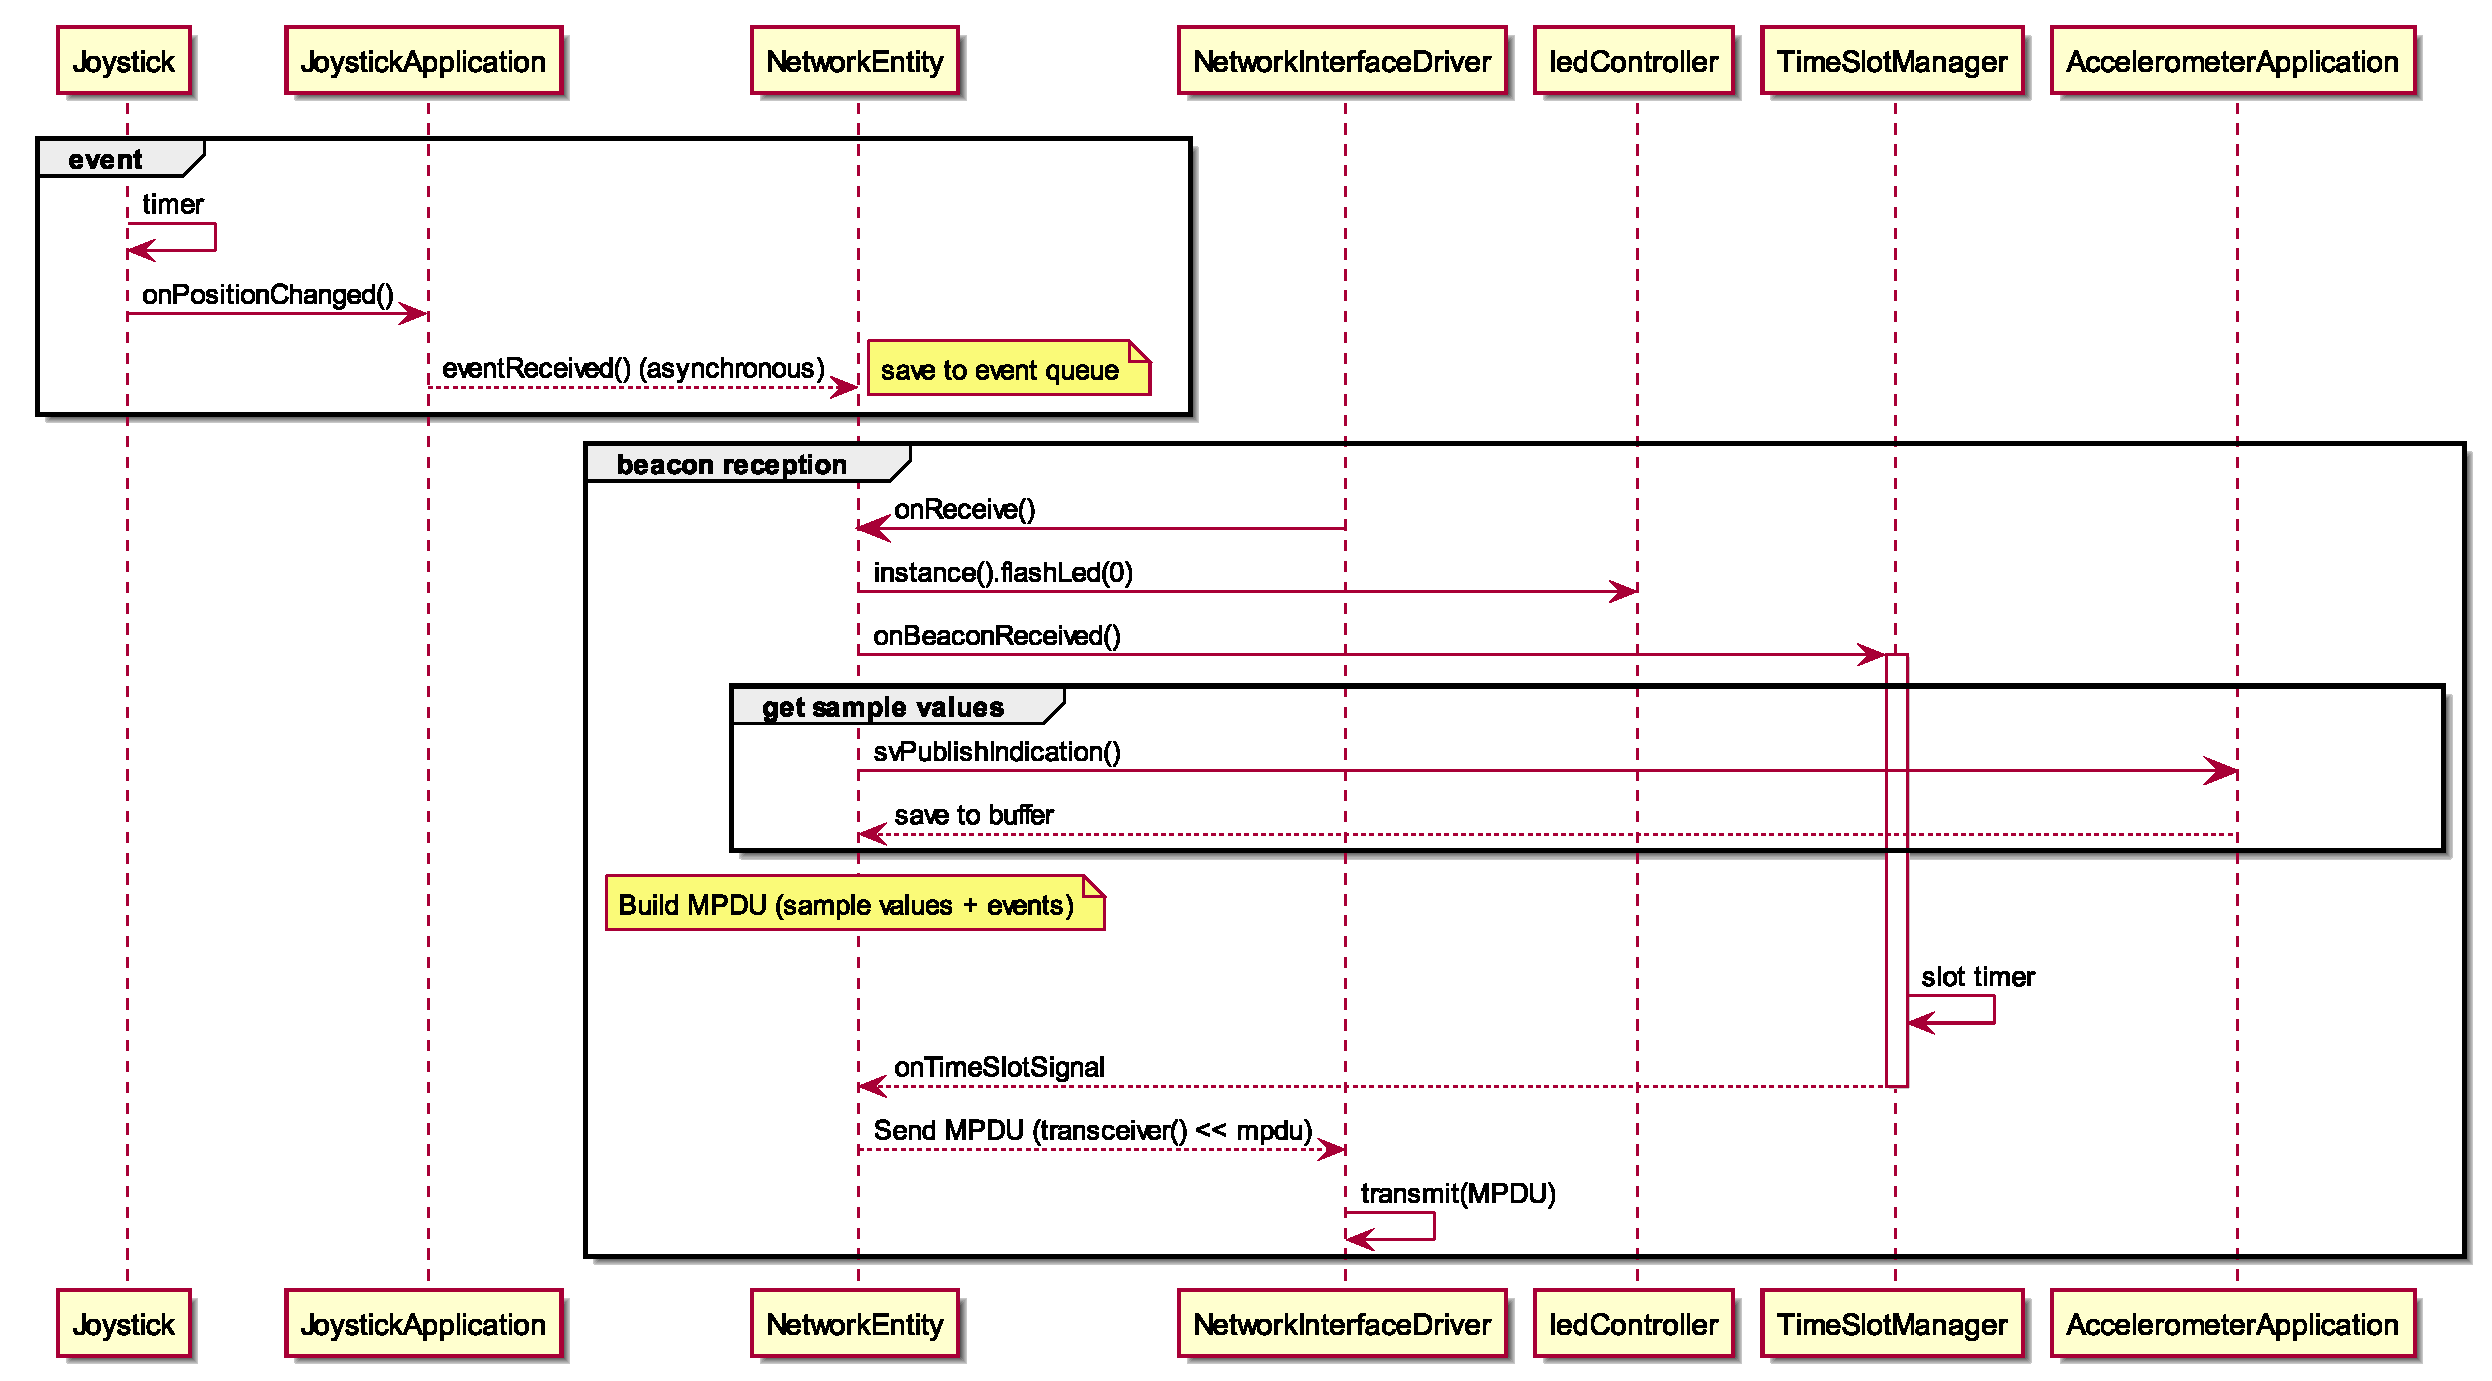
\includegraphics[width=0.9\textwidth]{out/sequence_beacon/sequence_beacon.eps}
\caption{Diagramme de séquence}
\end{figure}
\subsection{MPDU}



La création d'un MPDU se fait de la manière suivante :
\begin{enumerate}
\item Reset
\item Ajout des sample values (accéléromètre)
\item Ajout des événements (jusqu'à ce qu'il n'y en ait plus ou que le buffer soit plein). Effectuer un "commit" après chaque événement
\item Finalisation
\end{enumerate}
Une fois qu'un MPDU est prêt, il est envoyé au moment où le temps du slot est atteint (slot timer).
\end{document}